\documentclass[9pt,twocolumn]{article} 
\usepackage{simpleConference}
\usepackage{subfigure}
\usepackage{times}
\usepackage{graphicx}
\usepackage{amssymb}
\usepackage{url,hyperref}
\usepackage{footmisc}

% set up tight list spacing
\usepackage{enumitem} 
\setlist{nolistsep,nosep}

% for toggles
\usepackage{etoolbox}

\newcommand {\studyquote}[1]{\em ``#1''\normalfont}

% CHANGE FROM TOGGLE TRUE TO TOGGLE FALSE FOR NON-ANONYMOUS RENDERING
% http://tex.stackexchange.com/questions/5894/latex-conditional-expression
\newtoggle{anonymous}
\togglefalse{anonymous}
%\togglefalse{anonymous}

% CHANGE FROM TOGGLE TRUE TO TOGGLE FALSE TO HIDE COMMENTS
\newtoggle{comments}
\toggletrue{comments}
%\togglefalse{comments}

% Comment region command (from Wesley Willett)
\usepackage[usenames]{color}
\usepackage[usenames,dvipsnames]{xcolor}
\iftoggle{comments} {
  %if we want to show comments
  \newcommand {\ben}[1]{{\color{violet}\bf{BZ: #1}\normalfont}}
  \newcommand {\ai}[1]{{\color{BrickRed}\bf{BH: #1}\normalfont}}
}{
  %if we don't want to show comments
  \newcommand {\ben}[1]{}
  \newcommand {\ai}[1]{}
}

%%% Local Variables: 
%%% mode: latex
%%% TeX-master: "report"
%%% End: 


\begin{document}

\title{Project PtOWSN: Modeling OpenWSN MAC Layer using Ptolemy II}

\author{
  Antonio Iannopollo, Ben Zhang\\
  EECS, UC Berkeley\\
  \{antonio, benzh\}@eecs.berkeley.edu
}

\maketitle
\thispagestyle{empty}

\begin{abstract}
The emerging of the {\em Internet of Things} paradigm poses new challenges on the side of new application development. The usual and comfortable assumption of unlimited available resources is not only no longer valid, but completely reversed. Planning the distribution grade and the energy footprint of an application running on multiple low power nodes is a key factor for a successful result.
In this project, we describe the modeling and implementation the OpenWSN MAC layer with Ptolemy II. This network layer implements the IEEE802.15.4e standard, a variant of IEEE802.15.4 in which a set of time synchronized nodes communicate each other according to a predefined schedule. 
The result of our work is a fine grained, executable model able to provide precise information about power consumption of a network of nodes running arbitrary applications. We also provide a preliminary study of a simple multi-hop data transmission application.
\end{abstract}

\section{Introduction}
We want to model the OpenWSN \cite{watteyne2012openwsn} stack using Ptolemy II \cite{davis1999overview}. Our goal is to provide a tool to estimate power consumption, scalability and network behavior of a WSN application in an early phase of the design process.

Once completed, this project will provide a two-fold contribution. First, it is going to augment the building blocks available to the Ptolemy community. This means Ptolemy will be used to design applications with a clear high level semantics, while being able to evaluate lower level details and their impact once the application is deployed. Second, we are providing a tool to help the OpenWSN community in the development process.

We are focusing on modeling the MAC layer of OpenWSN. This layer implements the IEEE 802.15.4e protocol standard, based on a time synchronized channel hopping technique. We decided to model this stack layer because each state of the protocol state machine is associated with a single state of the radio. Modeling power consumption dynamics is, in this way, straightforward (we refer to \cite{vilajosana2013realistic} for details). Moreover, at this level it is possible to capture point to point communication issues and the impact of a network schedule, required by 802.15.4e. 

%%% Local Variables: 
%%% mode: latex
%%% TeX-master: "report"
%%% End: 

\section{Background on OpenWSN}
\label{sec:background-openwsn}

In this section, we provide a brief overview of the OpenWSN protocol stack. Interested readers can read \cite{watteyne2012openwsn, IEEE802.15.4e} and visit OpenWSN website\footnote{https://openwsn.atlassian.net/wiki/} for more information. 

{\bf Slotframe:} IEEE802.15.4e defines a {\em slotframe} structure. A slotframe is a group of temporal slots which is repeated over time. Current OpenWSN implementation uses 15ms slots. A {\em schedule} tells the node whether it should transmit, receive or sleep in a particular slot. The construction of such schedule if out of the scope of IEEE802.15.4e.

{\bf Time Synchronization:} When a node joins a network, it aligns its slot boundary with other nodes (slot synchronization) and set its Absolute Slot Number (ASN) to the network ASN (ASN synchronization). In this way, all nodes will enter in a new slot at the same time (following their pre-defined schedule). 

{\bf Re-synchronization:} Since the clock on the embedded platforms is not perfect (typical clock drift is around 10 parts-per-million (ppm)), a re-synchronization mechanism is needed. OpenWSN performs re-synchronization whenever a packet transmission happens. Each node picks as reference the neighbor that is closer to the root of the network as its time master, and the synchronization is achieved by aligning its next slot boundary to the master's. When there is no packet transmission, a {\em KeepAlive} packet is generated (every 30 seconds is a typical value).

{\bf OpenWSN State Machine:} In each slot, given the schedule, the node behaves according to a state machine. This state machine defines how the synchronization is reached and maintained, as well as transmission and reception. We defer the discussion here because this will be the main focus of our modeling work described in the next section.

{\bf Packet format:} the OpenWSN stack defines several types of packet. In our work, we consider three of them, related to the MAC layer: \texttt{ADV}, \texttt{DATA}, \texttt{ACK}. The advertisement packet \texttt{ADV} is used to broadcast the network information (such as ASN) such that new node can join the network. The \texttt{DATA} packet encapsulates the upper layer payload. The \texttt{ACK} packet is used to acknowledge a data packet. It also contains time correction information such that the other node can perform re-synchronization (if needed).


%%% Local Variables: 
%%% mode: latex
%%% TeX-master: "ee219d"
%%% End: 


\section{Modeling in Ptolemy}
\label{sec:modeling-ptolemy}

In this section, we present our work in Ptolemy that models the MAC layer of OpenWSN\footnote{Though the model in each figure is vector graphics, you can zoom in and read the details. We strongly suggest reader to open our Ptolemy model for details. These figures are mainly for illustration purpose.}.

\begin{figure}[t]
\centering
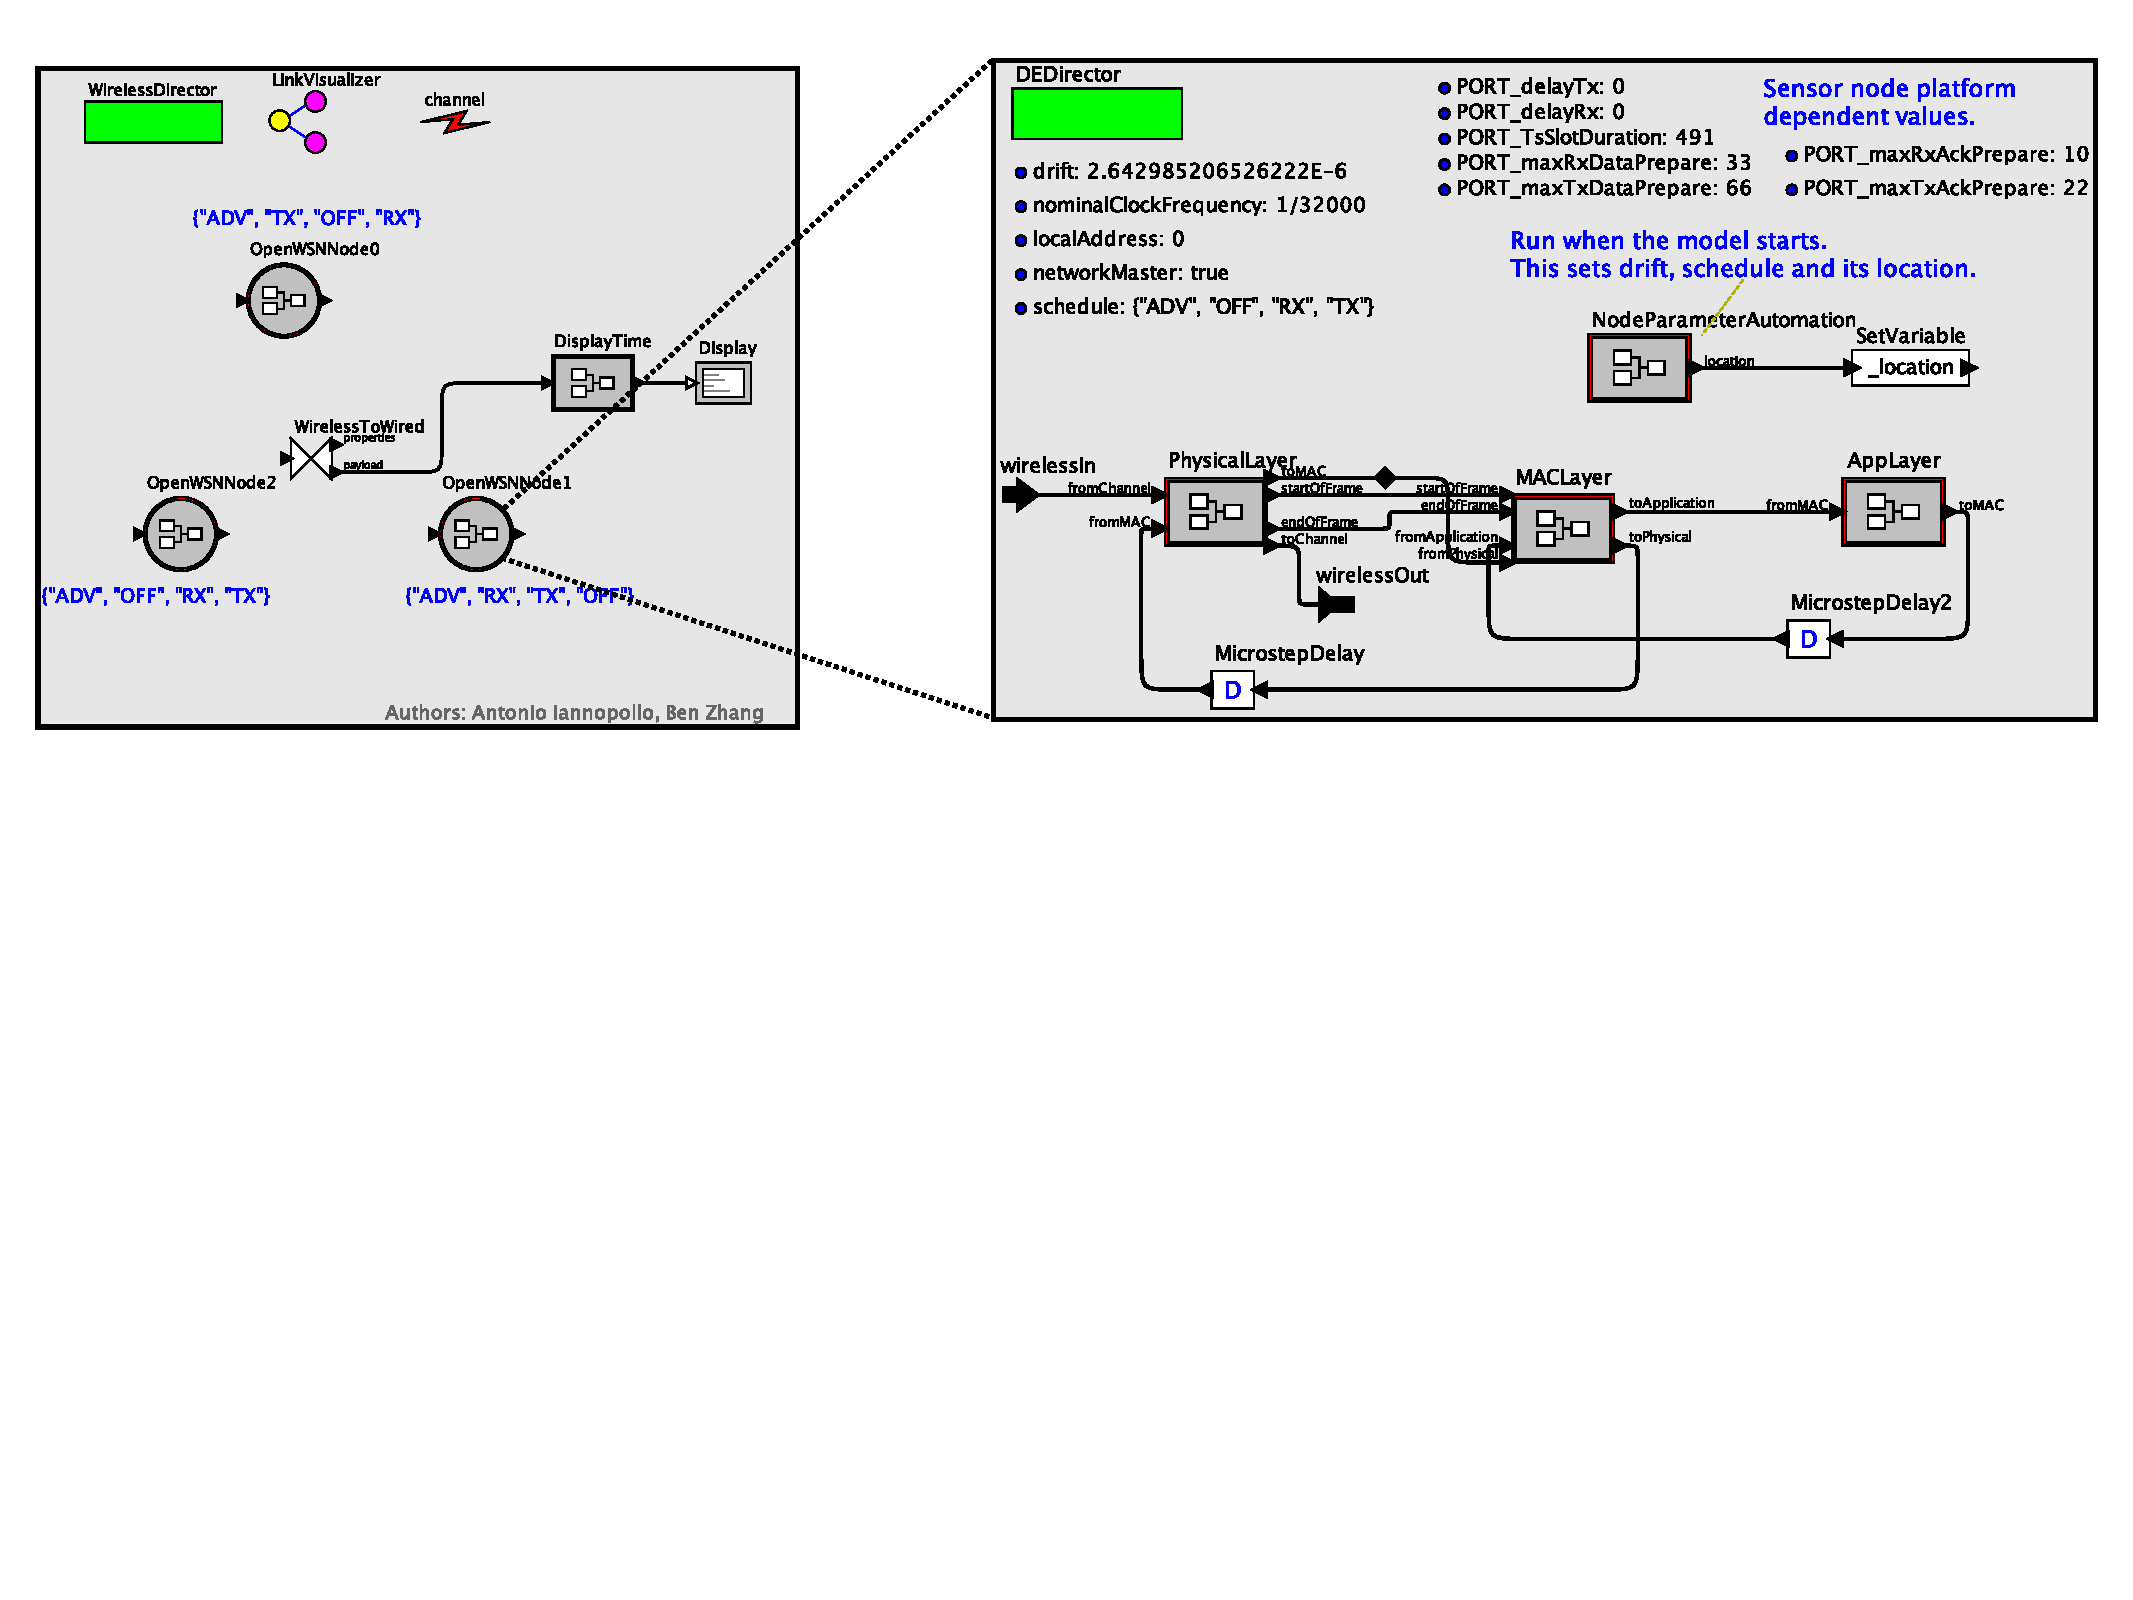
\includegraphics[width=1\columnwidth]{figures/PaperOpenWSNNode}
\caption{An example application of three nodes ({\em left}) and the simplified network stack ({\em right}).}
\label{fig:OpenWSNNode}
\end{figure}

Though our focus is on the TSCH state machine, we have also modeled a simple physical radio and abstracted the higher network layers as a single application layer (see Figure~\ref{fig:OpenWSNNode}). The interface to the Physical layer is mainly achieved with 1) \texttt{startOfFrame} and \texttt{endOfFrame} ports, which indicate the radio status; 2) \texttt{fromPhysical} and \texttt{toPhysical}ports, which convey the payload. The interface to the Application layer is through \texttt{fromMAC} and \texttt{toMAC} ports. 

Inside the \texttt{MACLayer} composite actor, we have a few actors including \texttt{packetQueueManager}, \texttt{scheduler}, \texttt{PacketProcessor} and \texttt{TSCHStateMachine} (names are self explanatory). The most relevant part is the \texttt{TSCHStateMachine}, where we modeled the protocol behavior using Hierarchical Modal Models \ref{fig:TSCHSM}. It consists of five main states, which describe the node activity: \texttt{init}, \texttt{SLEEP}, \texttt{synchronization}, \texttt{tx} and \texttt{rx}. 


\begin{figure}[t]
\centering
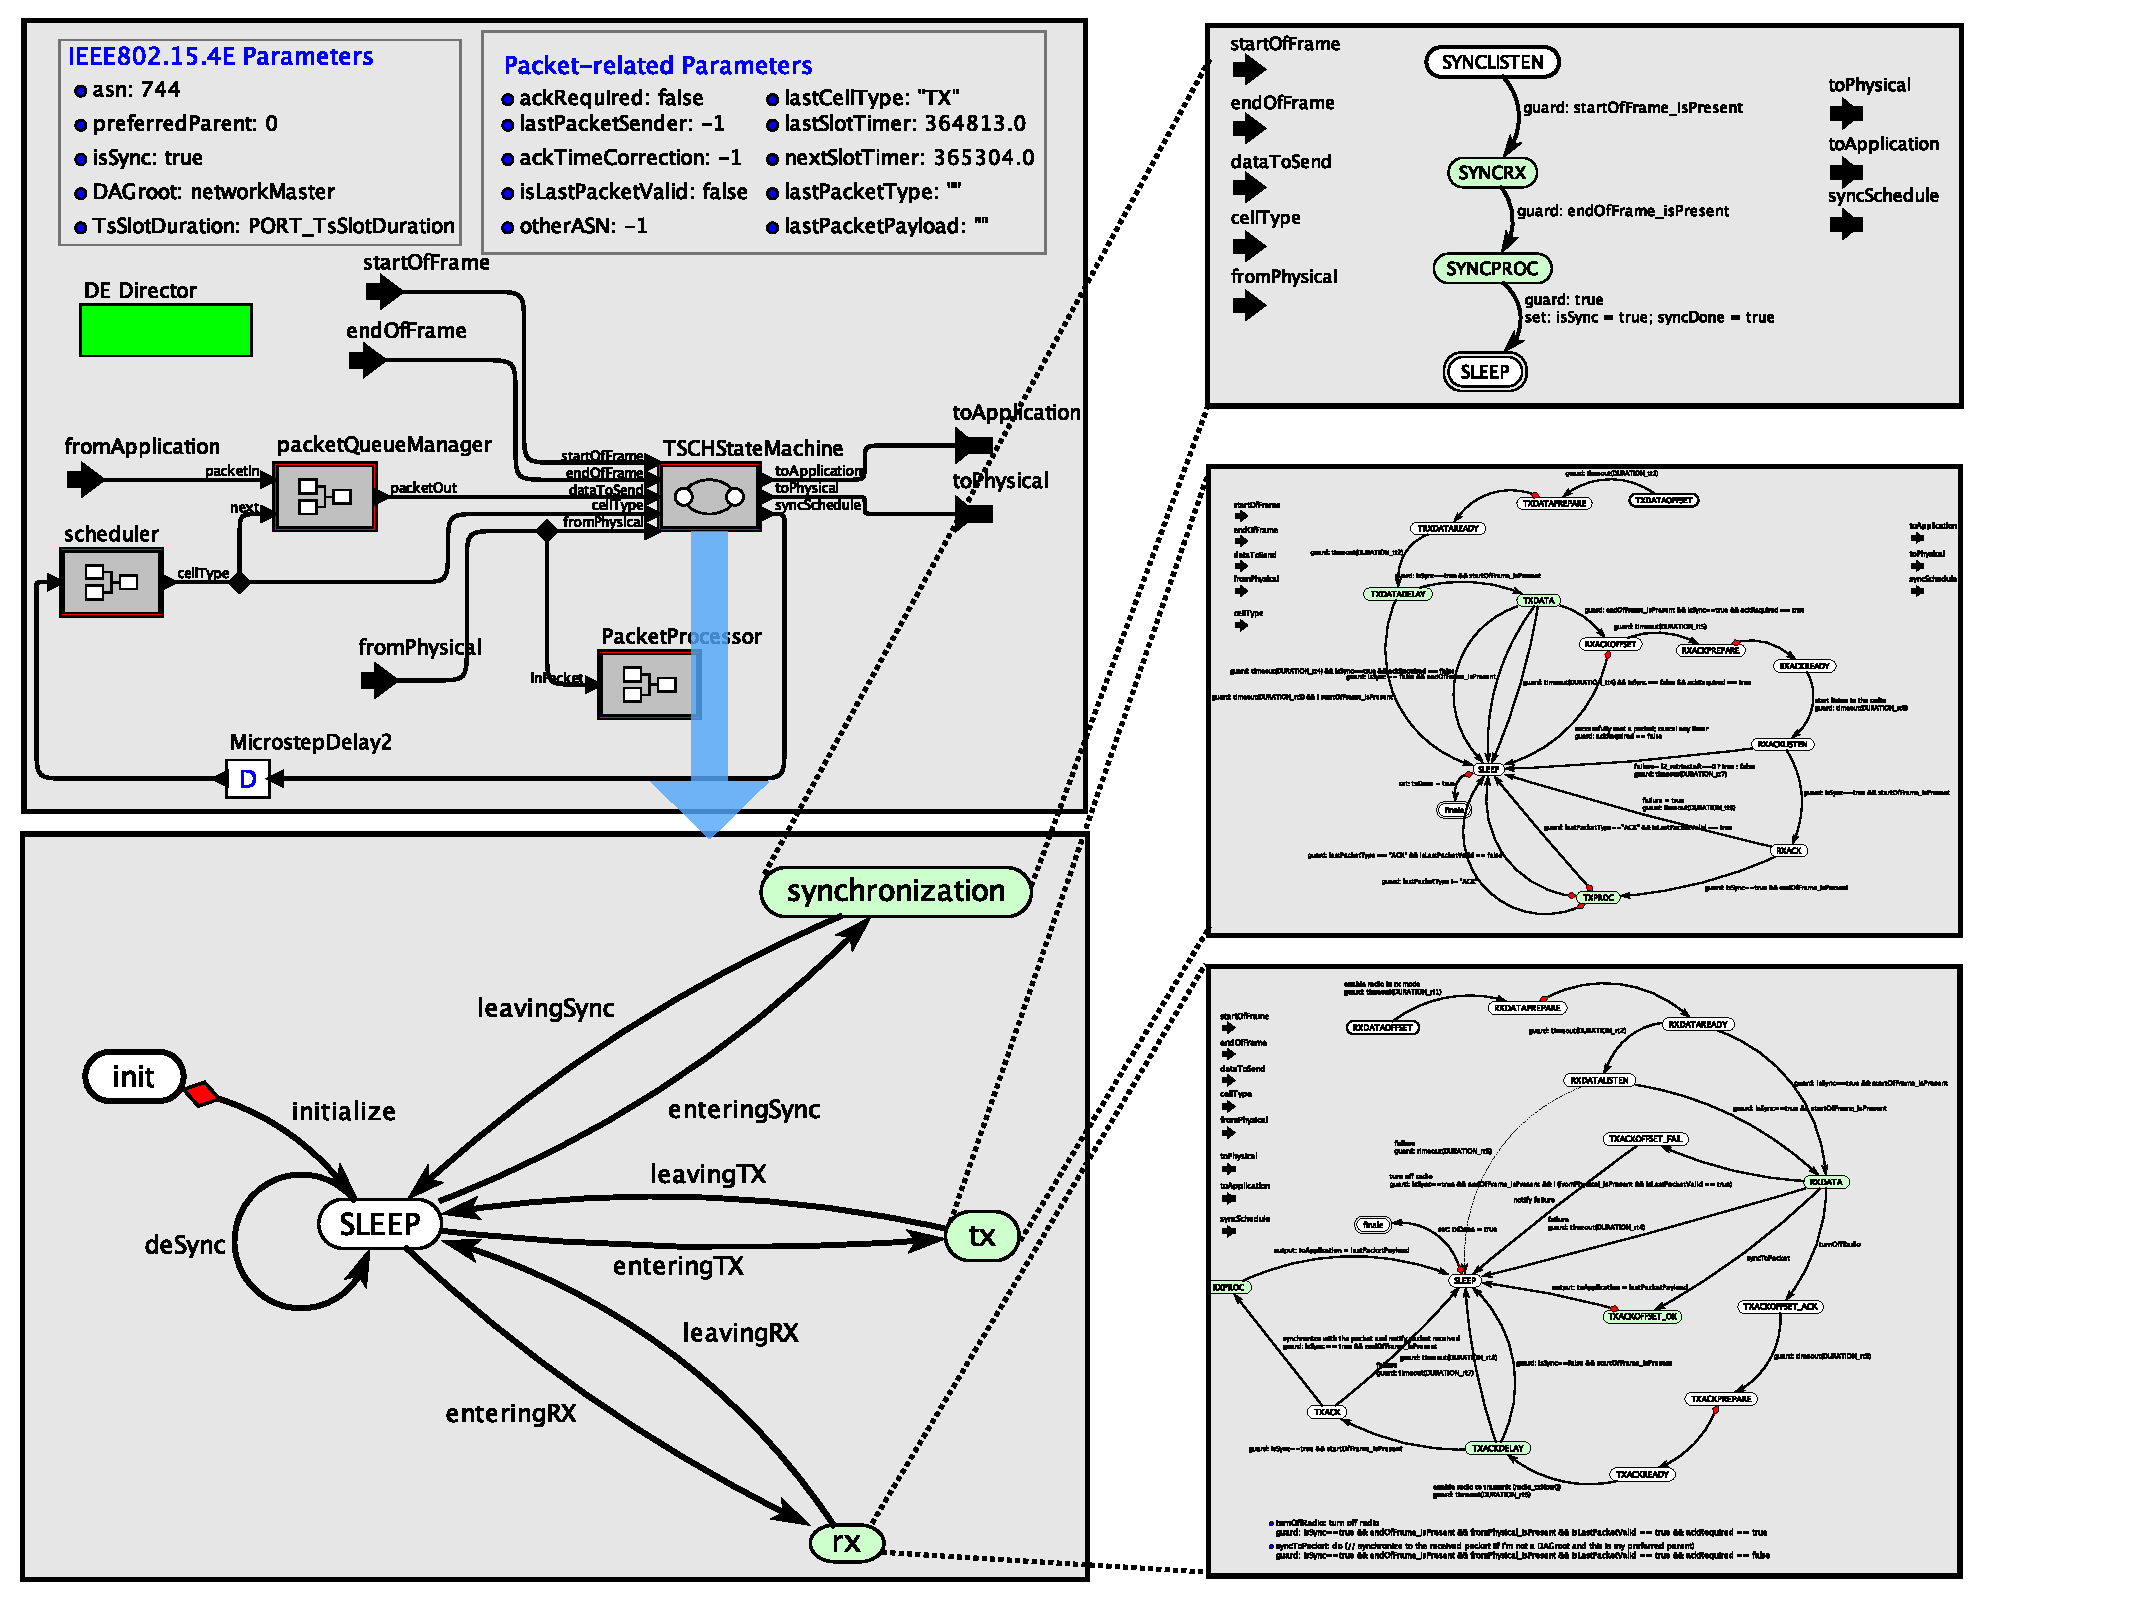
\includegraphics[width=1\columnwidth]{figures/PaperTSCHStateMachine}
\caption{The state machine with refinements of TSCH protocol.}
\label{fig:TSCHSM}
\end{figure}

During the initialization phase, we reset all protocol related parameters, When in the \texttt{synchronization} refinement, the node keeps listening for \texttt{ADV} packet and performs slot synchronization and ASN synchronization. Once the synchronization is done, it goes back to \texttt{SLEEP} state.
The scheduler decides node actions: 
\begin{itemize}
\item If the slot is \texttt{ADV} slot, then the node enters the \texttt{tx} state and sends an \texttt{ADV} packet. 
\item If it's \texttt{TX} or \texttt{RXTX} slot and the node has data to send (there are packets queued at \texttt{packetQueueManager}), it will enter \texttt{tx} state and send the data packet. 
\item If it's \texttt{RX} slot, or it's \texttt{RXTX} slot but the application doesn't have data to send, the node will enter \texttt{rx} state and listen for packets.
\end{itemize}

In \texttt{tx} and \texttt{rx} states, there is a refinement which captures the complicated state transition of the radio. For example, when the node is sending a packet, it first wait a certain time (in \texttt{TXDATAOFFSET} state), then prepares the data for radio to transmit (\texttt{TXDATAPREPARE}), and after a few other states that are used to check the radio status, etc., it finally enters \texttt{TXDATA} state and transmits the packet. Similar complexity exists for managing acknowledgment and receiving a packet. Given our space constraints, we refer the reader to our Ptolemy model for more details on state transition behavior.

The \texttt{synchronization} state is only entered when the node is not synchronized to the rest of the network anymore. Additionally, for every received packet, the node will capture the reception time (Figure~\ref{fig:timeCorrection} {\em up}). If the packet is from a time master, it will calculate the time discrepancy and use it to adjust its synchronization (Figure~\ref{fig:timeCorrection} {\em middle}). If the packet is from a time slave, then the node will still perform a calculation and send the time correction through \texttt{ACK} packet (Figure~\ref{fig:timeCorrection} {\em down}).

\begin{figure}[t]
\centering
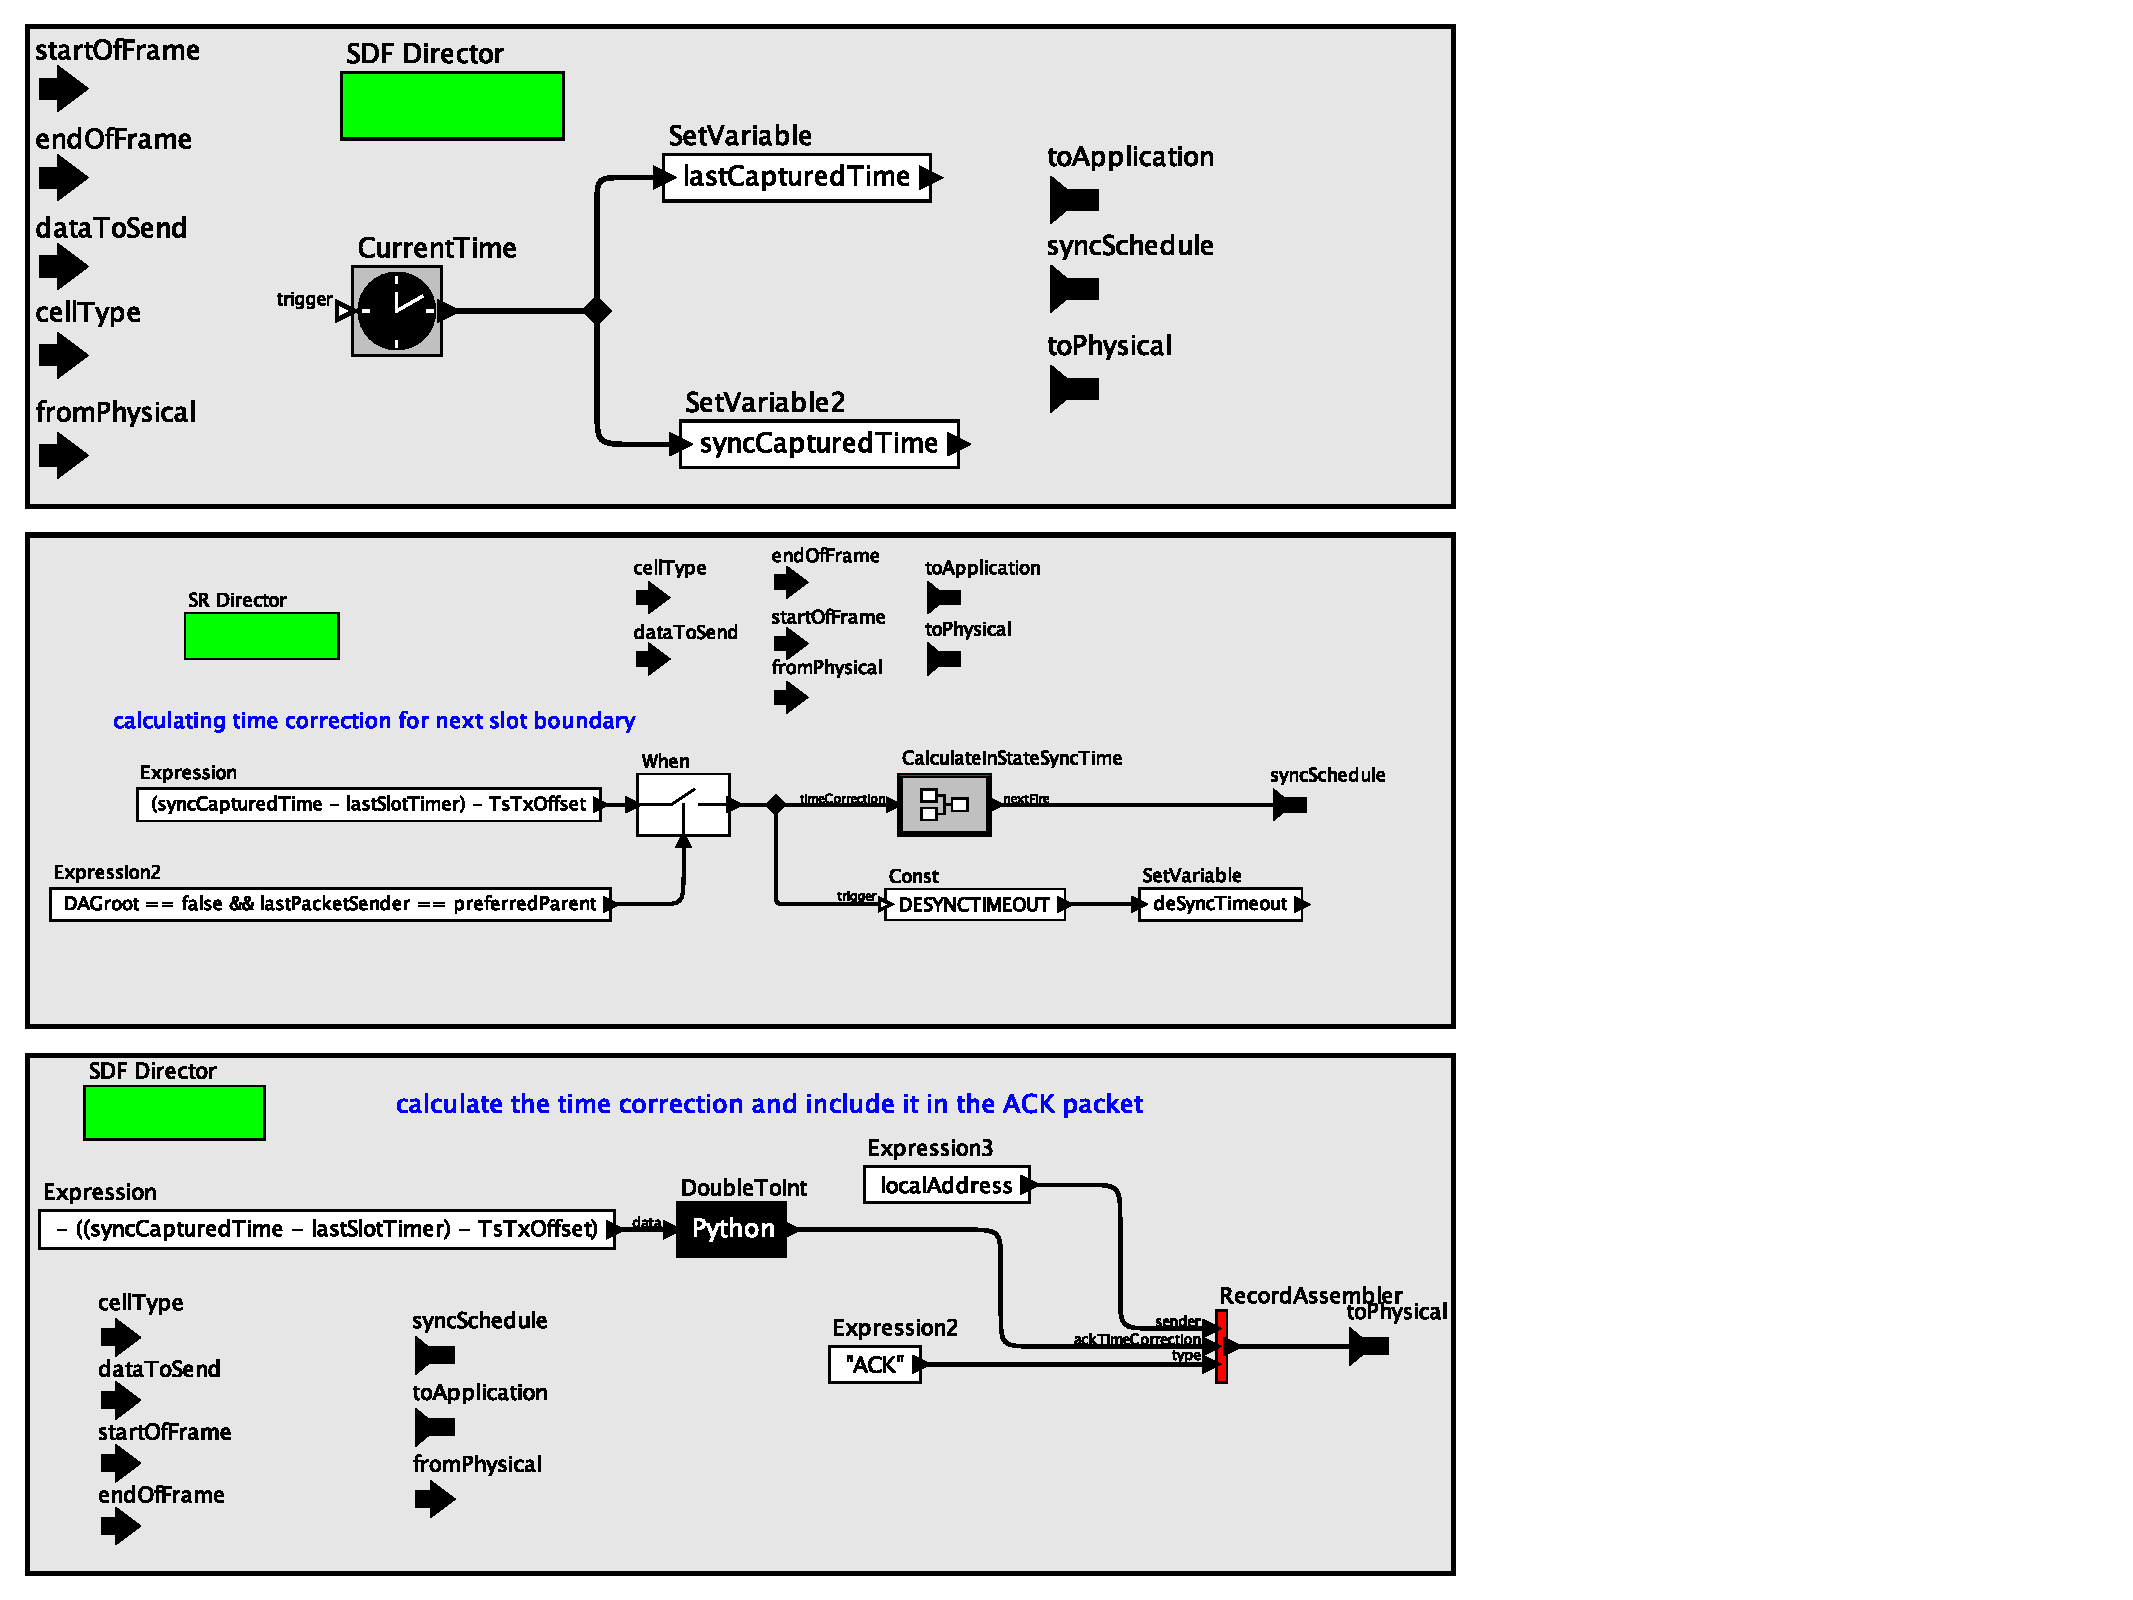
\includegraphics[width=0.9\columnwidth]{figures/PaperReSynchronization}
\caption{Modeling the the re-synchronization.}
\label{fig:timeCorrection}
\end{figure}

%%% Local Variables: 
%%% mode: latex
%%% TeX-master: "ee219d"
%%% End: 

\section{Case Study}
\label{sec:case-study}

We consider a multi-hop network which has a chain of OpenWSN nodes (see Figure~\ref{fig:multihop}), where each node has a different {\em NodeId} (assigned as an integer), increasing from left to right. 
\begin{figure}[t]
\centering
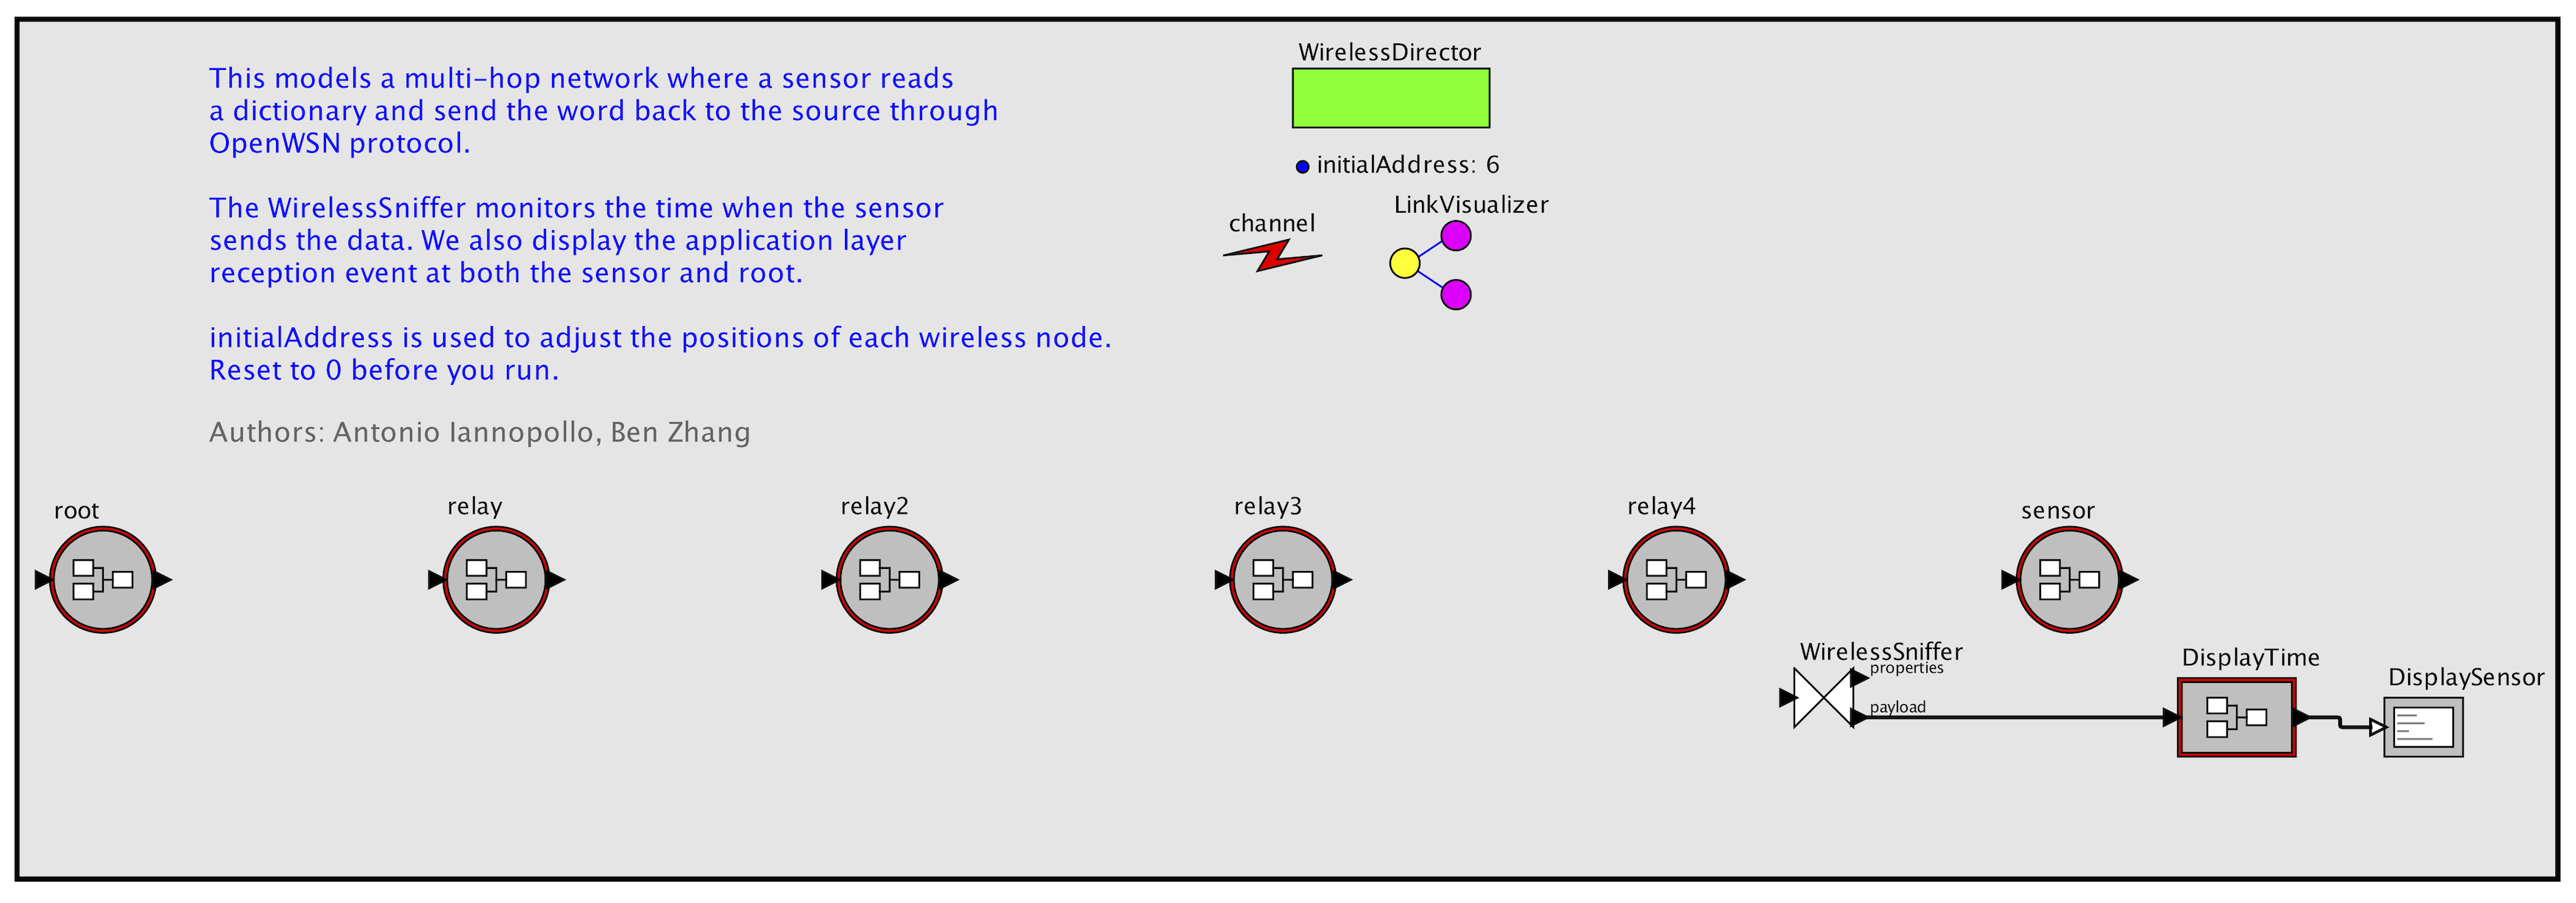
\includegraphics[width=1\columnwidth]{figures/PaperDemoPtolemy}
\caption{A multi-hop OpenWSN network.}
\label{fig:multihop}
\end{figure}
Node schedules are constructed following the schema\footnote{Interestingly, we are inspired by Gustove function to came up with such a schedule so that at any given time, a node is communicating only with one of its neighbors such that there will not be hidden terminal problem if time synchronization is achieved.}:

\begin{tabular}{ l | c | c | c | c | c }
  \hline                       
  NodeId & \multicolumn{5}{c}{Schedules} \\
  \hline
  $3i+0$ & \texttt{ADV} & \texttt{TX} & \texttt{RX} & \texttt{OFF} & $k \times \texttt{OFF}$ \\
  $3i+1$ & \texttt{ADV} & \texttt{RX} & \texttt{OFF} & \texttt{TX} & $k \times \texttt{OFF}$ \\
  $3i+2$ & \texttt{ADV} & \texttt{OFF} & \texttt{TX} & \texttt{RX} & $k \times \texttt{OFF}$ \\
  \hline  
\end{tabular}
where $i \in \mathbb{N}$ and $k$ is specified to control the duty cycle of each node (higher $k$ indicates more \texttt{OFF} in the schedule period and thus a lower duty cycle). Intuitively, when $k$ is small, nodes can receive \texttt{ADV} packet in a relatively timely fashion. This helps especially in case of lost synchronization. However, in case of high duty cycle schedules, the price a node needs to pay is to spend more time in \texttt{TX} and \texttt{RX} states, which potentially increases the power consumption. On the other hand, if $k$ is large, nodes that have lost synchronization will have to wait longer, leading to an increased energy consumption caused by turning the radio on and listening for long periods. Schedule duty cycle tuning is a critical activity in order achieve performance while minimizing energy consumption. In this work, we leave a formal study as future work, and only focus on cases when $k = 0, 144, 306$.

\begin{figure}
\hfill
\subfigure[For each node, the time it first get synchronized (the time it joins the network).]{ 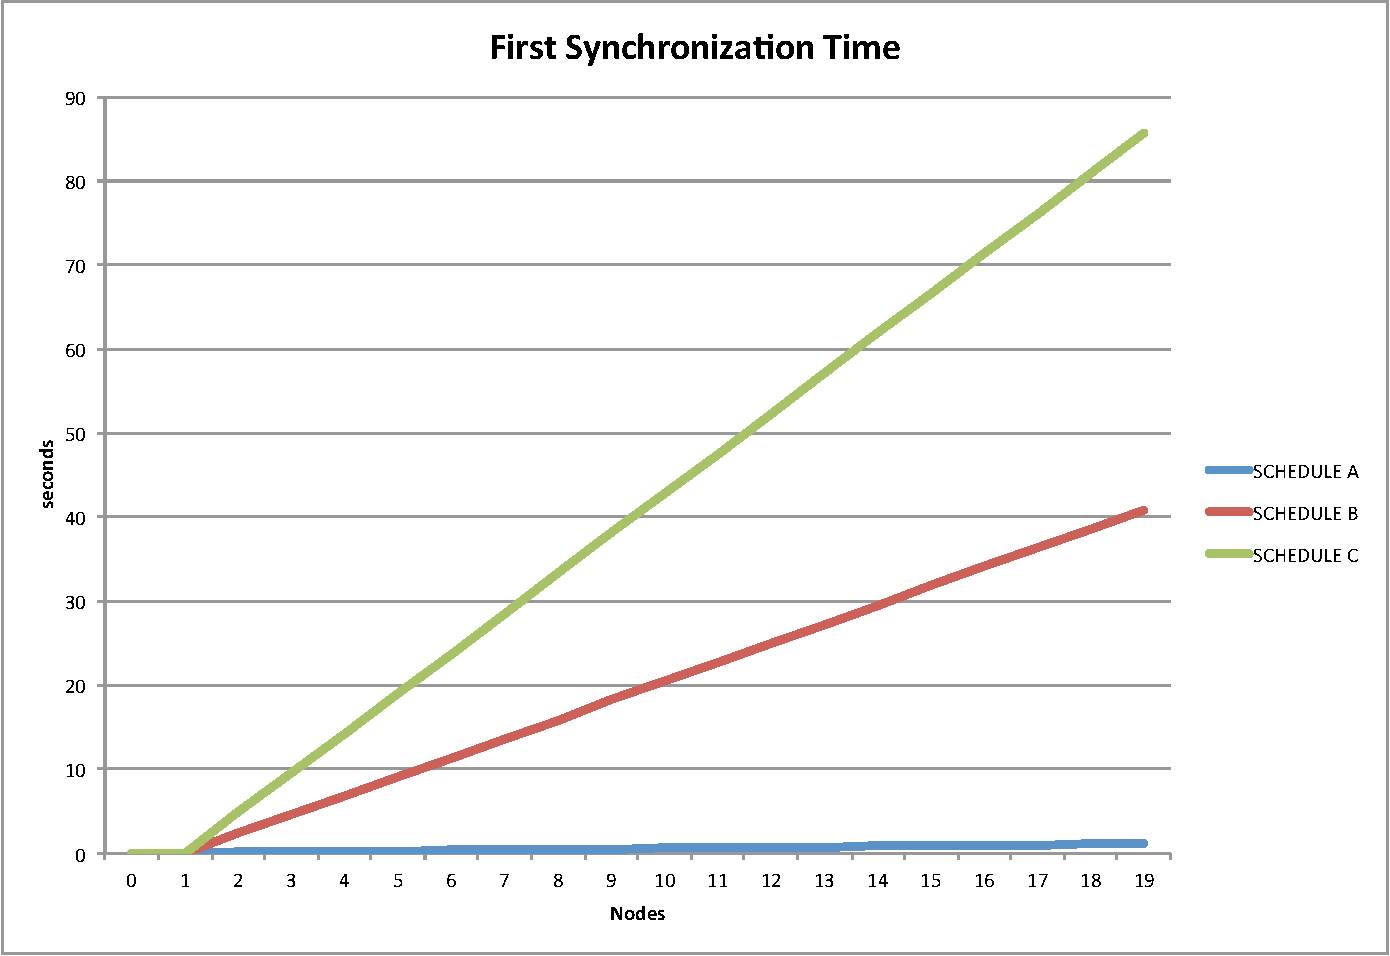
\includegraphics[width=.45\linewidth]{figures/synch_time_sched}}
\hfill
\subfigure[For each node, the measured power consumption after then network is on for 20 seconds.]{ 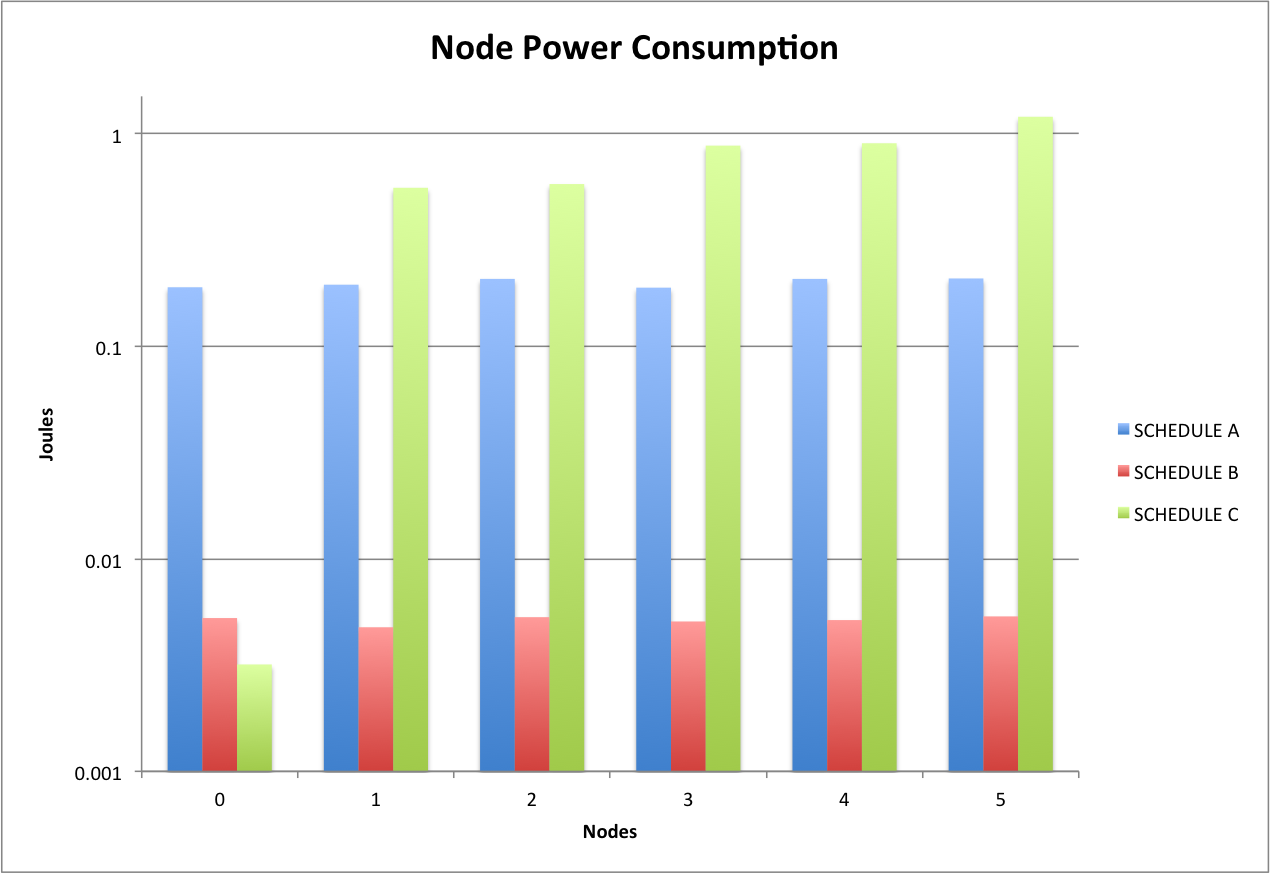
\includegraphics[width=.45\linewidth]{figures/power_cons}}
\hfill
\caption{Performance evaluation for different schedules in a multi-hop network. Schedule A, B, C are corresponding to $k = 0, 144, 306$.}
\label{fig:evaluation}
\end{figure}

We present the results of a network that has 6 chained nodes\footnote{The first synchronization figure was obtained with a simulation of 20 nodes. Given that the linear relationship is clear, we present the graph with 6 nodes for consistency with the power consumption results.} under the three different schedules in Figure~\ref{fig:evaluation}; and use two metrics to evaluate each schedule. The first metric is the time of first synchronization for each node in the network. This metric gives us an idea of how \emph{reactive} the network is. The second is the power consumption of each node in the network for a given period of time. This helps to evaluate the overall lifetime of network devices, which correlates to the network {\em durability}.

Keeping looking at Figure~\ref{fig:evaluation}, on the left, we see that the first synchronization time is proportional to the relative distance of each node from the root (as the reader intuition suggests). In case of higher duty cycle, when $k$ is smaller (such as with Schedule A), each node waits for a shorter time to reach synchronization. 

From the power consumption side (figure on the {\em right}), we have found that if the duty cycle is high ($k$ is small), then most nodes are busy in \texttt{TX} and \texttt{RX} states, leading to similar energy consumption values. When the duty cycle is low, then nodes that are farther from the root tend to stay longer in the \texttt{synchronization} state (because of the less frequent \texttt{ADV} packets), resulting in longer times with the radio in listening mode. Interestingly, schedules with a moderate duty cycle (see Schedule B), where transmissions are less frequent but not in a way to cause node de-synchronization, lead to an overall smaller amount of energy consumption. 

%%% Local Variables: 
%%% mode: latex
%%% TeX-master: "ee219d"
%%% End: 


\section{Conclusion}
\label{sec:conclusion}

Work is proceeding smoothly following our previous roadmap (with minor changes). We are extending our model according to an iterative approach, which allows us to capture feedback and fix issues while improving its functionality. By the end of the month, we plan to simulate inter-node communication and time synchronization, tag each execution with a specific power consumption index.



%%% Local Variables: 
%%% mode: latex
%%% TeX-master: "report"
%%% End: 


\bibliographystyle{abbrv}
{\footnotesize \bibliography{ee219d}}

\appendix
\section{Demos}

We have constructed two demos that can serve the purpose of understanding the time synchronization and multi-hop data transmission in OpenWSN protocol. They are named \verb+demo_multihop_dict_nopower.xml+(see Figure~\ref{fig:multihop}) and \verb+demo_sync.xml+(see Figure~\ref{fig:timesync}) in the accompanying folder with this report. Readers are welcome to open it and run it with Ptolemy II. 

\begin{figure}[t]
\centering
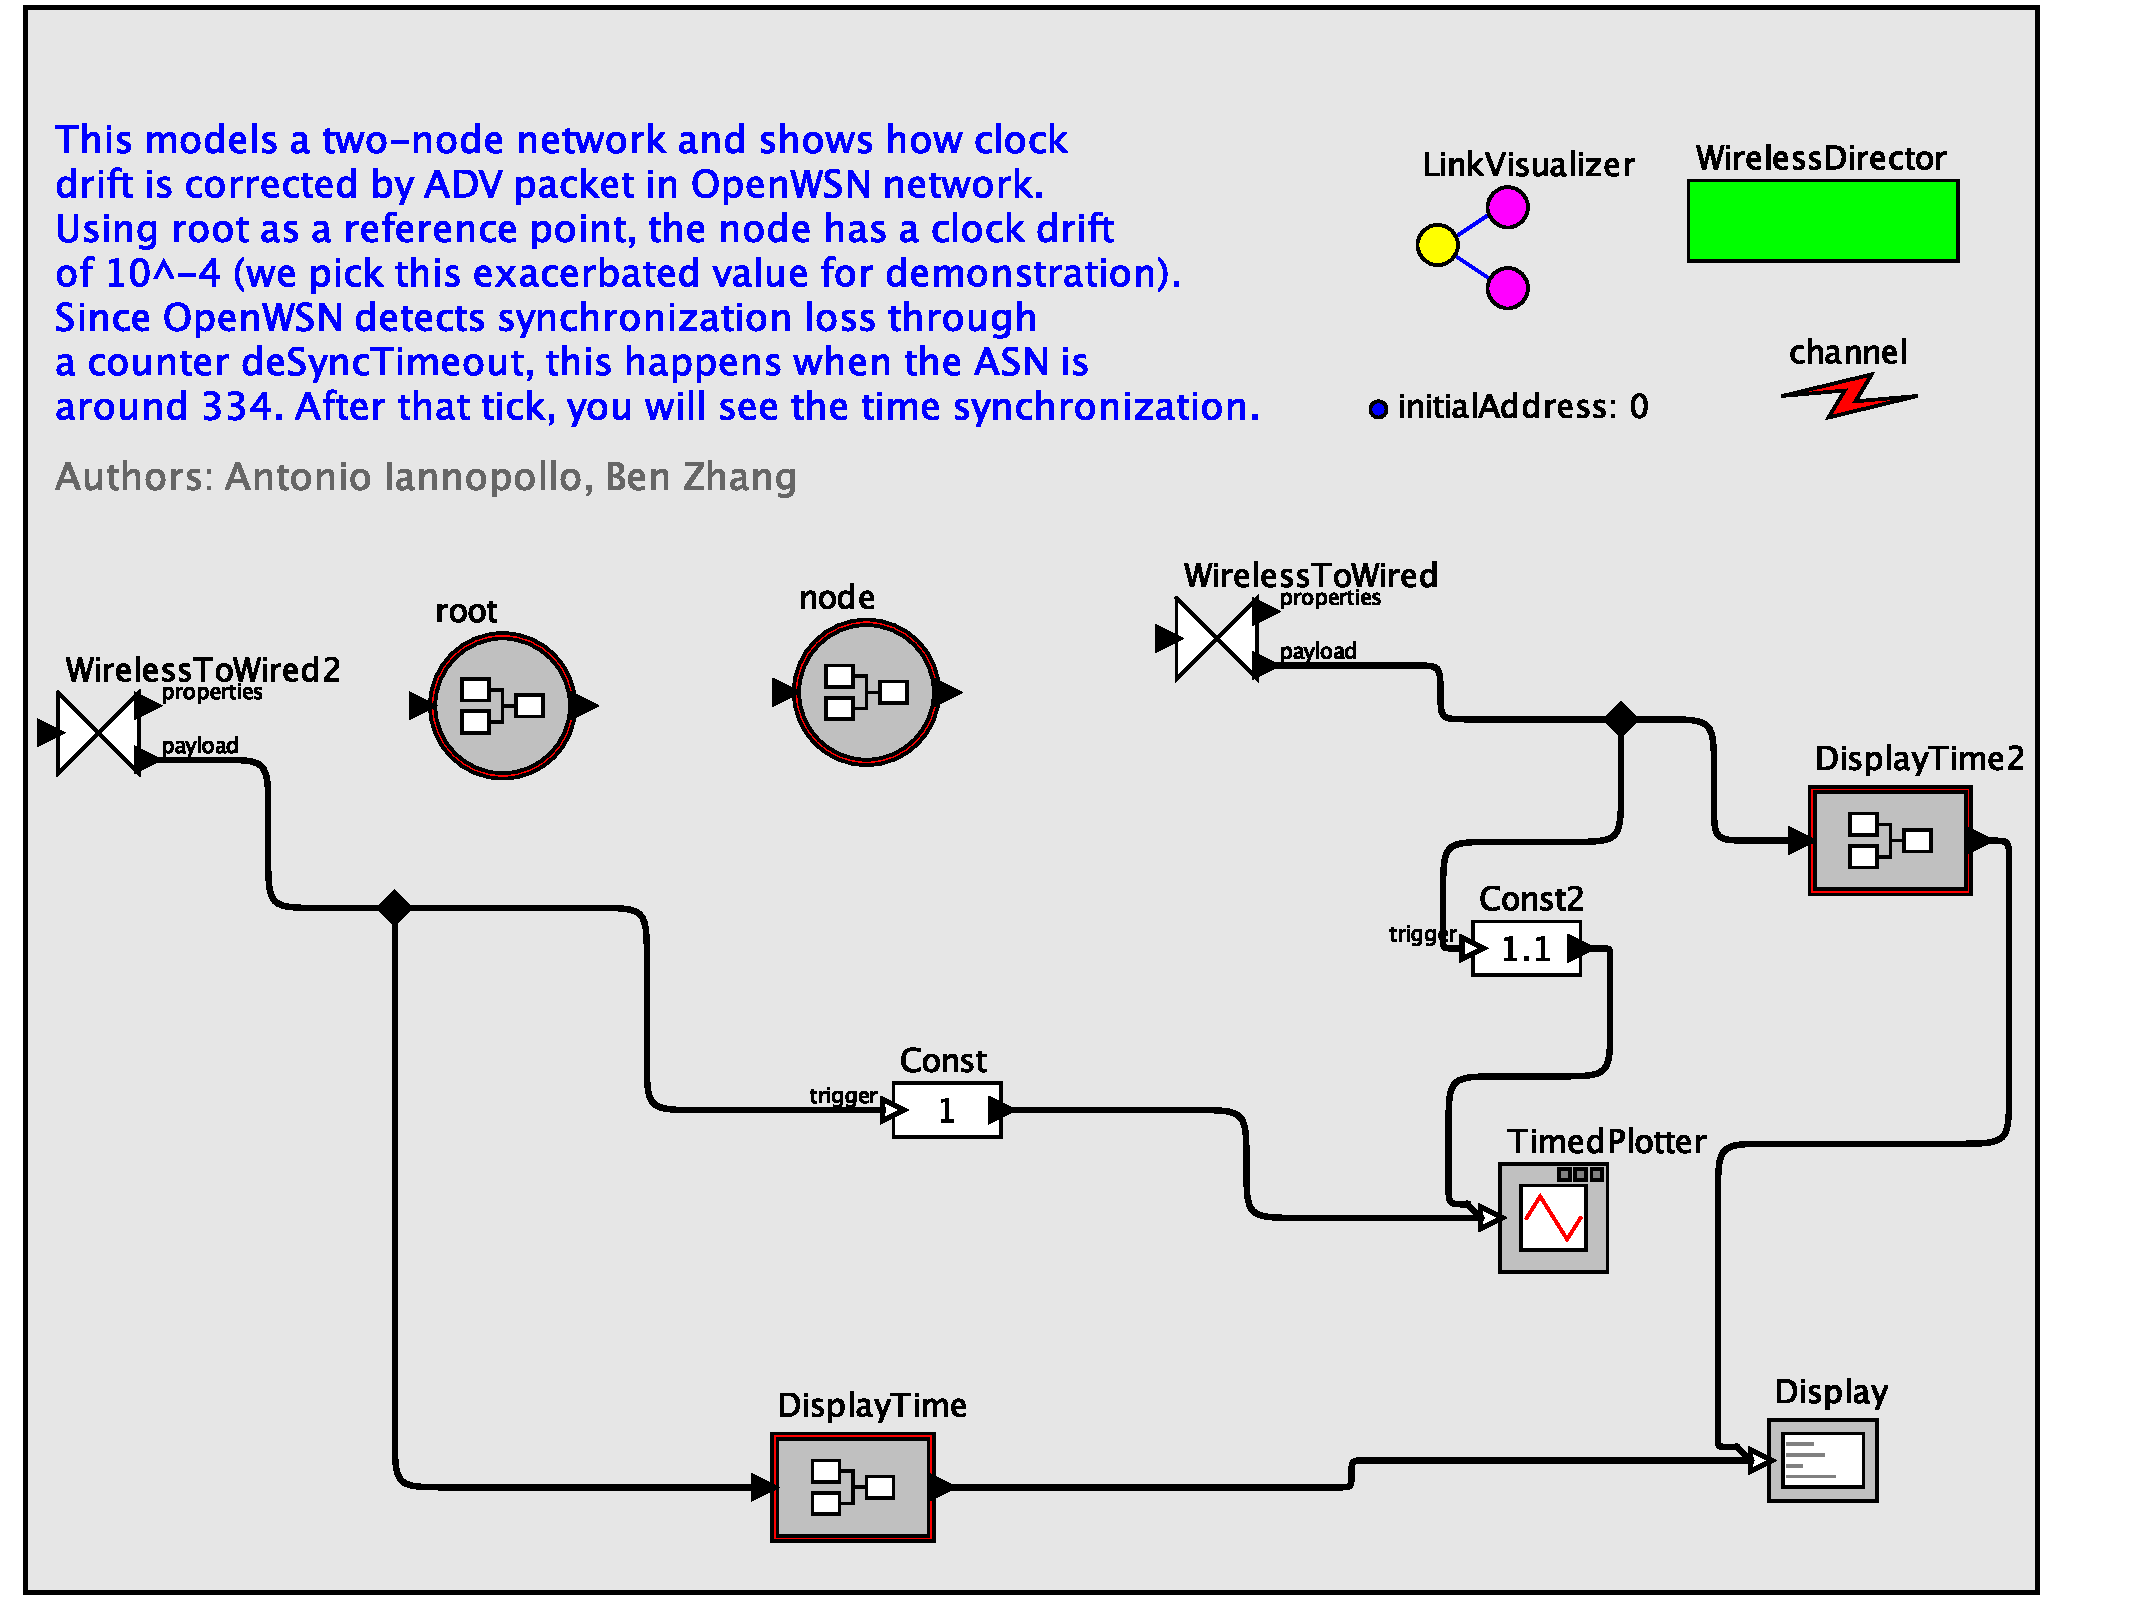
\includegraphics[width=0.9\columnwidth]{figures/PaperDemoSync}
\caption{\small Ptolemy demo that shows the action of time synchronization.}
\label{fig:timesync}
\end{figure}


%%% Local Variables: 
%%% mode: latex
%%% TeX-master: "ee219d"
%%% End: 


\end{document}
